\setcounter{aufgabe}{0}

\begin{aufgabe}{Prozente -- rechnen und umrechnen. Rechne, wo es geht, im Kopf.}
\begin{teile}
\teil 30 von 100 Stiften sind rot. \feld[\%]{p}
\teil 7 von 100 Feldern sind grau. \feld[\%]{p}
\teil Schreibe als Prozent: $0{,}45$ \leerfeld[\%]
\teil Schreibe als Dezimalzahl: $8\,\%$ \leerfeld
\teil 12 von 48 Kindern haben ein Instrument gelernt. \feld[\%]{p}
\teil In einer Klasse fahren $45\,\%$ mit dem Rad und $30\,\%$ mit dem Bus, der Rest geht zu Fuß. \feld[\%]{p}
\end{teile}
\end{aufgabe}

\begin{aufgabe}{Zahlen ordnen und Skalen ablesen.}
Ordne von klein nach groß.
\begin{teile}
\teil $4{,}7 \quad 4{,}07 \quad 4{,}71 \quad 4{,}17$ \\[2pt] \leerfeld\ $<$ \leerfeld\ $<$ \leerfeld\ $<$ \leerfeld
\teil $12{,}5 \quad 9{,}8 \quad 12{,}05 \quad 9{,}75$ \\[2pt] \leerfeld\ $<$ \leerfeld\ $<$ \leerfeld\ $<$ \leerfeld
\end{teile}

Lies die Zahlen am Zahlenstrahl ab.

\zahlenstrahl[xmin=0,xmax=5,xstep=0.5,karo=1.4]{1.5/A, 3.25/B, 4.75/C}

\begin{teilezwei}
\tz $A =$ \leerfeld & \tz $B =$ \leerfeld \\
\tz $C =$ \leerfeld & \\
\end{teilezwei}
\begin{teile}
\teil Auf einer Achse sind die Linien mit $0$, $50$, $100$, $150$ beschriftet. Zwischen zwei beschrifteten Linien liegen vier dünne Hilfslinien. Wie viel ist ein Schritt von Linie zu Linie wert? \leerfeld
\end{teile}
\end{aufgabe}

\begin{aufgabe}{Winkel und Anteile am Vollkreis.}
\begin{teile}
\teil Ein Vollkreis hat \leerfeld[$^\circ$]
\teil Ein Viertel des Vollkreises: \leerfeld[$^\circ$]
\teil Die Hälfte des Vollkreises: \leerfeld[$^\circ$]
\teil Ein Drittel des Vollkreises: \leerfeld[$^\circ$]
\teil Ein Zehntel des Vollkreises: \leerfeld[$^\circ$]
\teil Ein Winkel misst $45^\circ$. Welcher Anteil des Vollkreises ist das? \leerfeld
\teil Trage am Strahl mit dem Geodreieck einen Winkel von $70^\circ$ an.
\end{teile}

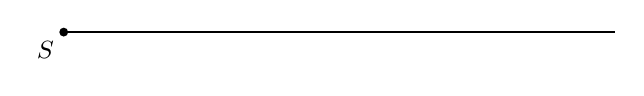
\begin{tikzpicture}
  \draw[line width=0.7pt] (0,0) -- (7,0);
  \fill (0,0) circle (1.6pt) node[below left,font=\small] {$S$};
\end{tikzpicture}
\end{aufgabe}

\begin{aufgabe}{Zentimeter und Millimeter.}
\begin{teilezwei}
\tz $3\,$cm $=$ \leerfeld[mm] & \tz $45\,$mm $=$ \leerfeld[cm] \\
\tz $7{,}2\,$cm $=$ \leerfeld[mm] & \tz $10\,$cm $=$ \leerfeld[mm] \\
\end{teilezwei}
\begin{teile}
\teil Trage auf der Linie vom linken Ende aus $6{,}5\,$cm ab und markiere die Stelle mit einem Strich.
\end{teile}

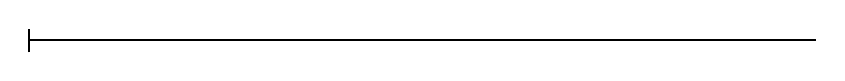
\begin{tikzpicture}
  \draw[line width=0.7pt] (0,0) -- (10,0);
  \draw[line width=0.7pt] (0,-0.15) -- (0,0.15);
\end{tikzpicture}
\end{aufgabe}

\begin{aufgabe}{Mit Dezimalzahlen rechnen und runden. Bei e) bis g) darfst du den Taschenrechner benutzen.}
\begin{teilezwei}
\tz $2{,}5 + 3{,}5 =$ \leerfeld & \tz $12 : 4 =$ \leerfeld \\
\tz $18{,}6 + 4{,}9 + 0{,}5 =$ \leerfeld & \tz $78 : 5 =$ \leerfeld \\
\tz $61{,}5 : 4 =$ \leerfeld & \\
\end{teilezwei}
\begin{teile}
\teil Runde dein Ergebnis aus e) auf eine Stelle nach dem Komma. \leerfeld
\teil Runde $3847{,}6$ auf Hunderter. \leerfeld
\end{teile}
\end{aufgabe}

\begin{aufgabe}{Bruchteil und Vielfaches einer Zahl.}
\begin{teilezwei}
\tz Die Hälfte von $60$: \leerfeld & \tz Ein Drittel von $90$: \leerfeld \\
\tz Ein Viertel von $70$: \leerfeld & \tz Doppelt so viel wie $45$: \leerfeld \\
\end{teilezwei}
\begin{teile}
\teil Ein Drittel mehr als $210$ -- wie viel ist das? \leerfeld
\teil Von den Befragten nennt jede fünfundzwanzigste Person Tennis. Wie viel Prozent sind das? \leerfeld[\%]
\end{teile}
\end{aufgabe}

\begin{aufgabe}{Fehler finden -- Anteile in Prozent.}
In einer Gruppe von 36 Jugendlichen haben 27 ein eigenes Fahrrad. Tim will wissen, wie viel Prozent das sind, und rechnet:
\rechnung{27 : 9 &= 3 \\ &= 300\,\%}
\begin{teile}
\teil Finde den Fehler, benenne ihn und schreibe die richtige Rechnung auf. \\[10pt]
\teil Von 60 Besuchern kaufen 21 ein Getränk. Wie viel Prozent sind das? \feld[\%]{p}
\end{teile}
\end{aufgabe}
